 \documentclass[a4paper,10pt]{article}
\usepackage[a4paper,top=3cm,bottom=3cm,left=2cm,right=2cm]{geometry}
\usepackage[pdftex=true,colorlinks=true,linkcolor=black,urlcolor=blue,plainpages=false]{hyperref}
\usepackage[utf8]{inputenc}
\usepackage[catalan]{babel}
\usepackage{graphicx}
\usepackage{subfigure}
\usepackage[rflt]{floatflt}
\usepackage{amssymb}
\pagestyle{headings}

\begin{document}
\begin{titlepage}
\title{\bf{INFORME PRÀCTICA 1 \\ XARXES II \\ MÀSTER EN ENGINYERIA DE P. L.}}
\author{Ignasi Barri Vilardell \\ Alberto Montañola Lacort \\ Josep Rius Torrentó}
\date{\today}
\maketitle
\thispagestyle{empty}
\pagebreak
\setcounter{page}{1}
\tableofcontents{}
\listoffigures
\listoftables
\pagebreak
\end{titlepage}

\pagebreak

\section{Introducció}
En aquest informe s'intenta mostrar una guia de les decisions preses pels tres integrants del grup alhora de resoldre la pràctica 1 de l'assignatura de \emph{Xarxes II} que està continguda dins del pla d'estudis del \emph{Màster en Enginyeria de Programari Lliure} que s'imparteix en l'\emph{Escola Politècnica Superior} dins de la \emph{Universitat de Lleida}.

	\subsection{Pretencions inicials de la pràctica}
	La pràctica que s'ens proposa, tracta la problemàtica d'implementar un \emph{xat}\footnote{Xat (català:conversa), que també es coneix amb el nom de conversa cibernètica, és un anglicisme que usualment es refereix a una comunicació escrita a través d'internet entre dues o més persones que es realitza de forma instantània.} usant una estructura de \emph{client-servidor}, això sí, seguint una sèrie de pecularietats imposades pel protocol que aquesta eina de comunicació haurà de seguir.

	A continuació farem un breu resum fent ús d'esquemes i diagrames que permetin situar al lector de les funcionalitats que la implementació d'aquesta eina ha de seguir, per tal de la seva correcta avaluació.

		\subsubsection{Accions de l'usuari}
		Un cop s'ha iniciat el \emph{servidor}, caldrà connectar el primer {client}, aquest, portarà a terme una configuració amb el servidor\label{configuracio}; aquest procediment es pot veure de forma esquemàtica en la figura \ref{config}.

			        \begin{figure}[h]
				\begin{center}
				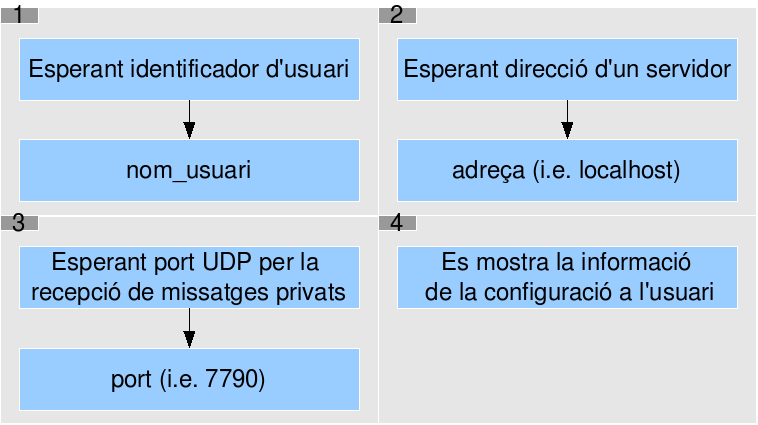
\includegraphics[scale=0.4]{config.png}
				\caption{Procés de configuració d'un client.}
				\label{config}
				\end{center}
				\end{figure}

		Acabat el procés de connexió, configuració i enregistrament del client, ja podem interactuar amb aquest, és a dir, enviar missatges, demanar ajuda, sortir del xat \ldots etc. Totes aquestes operacions, queden reflexades en l'esquema de la figura \ref{user_actions}.

			        \begin{figure}[h]
				\begin{center}
				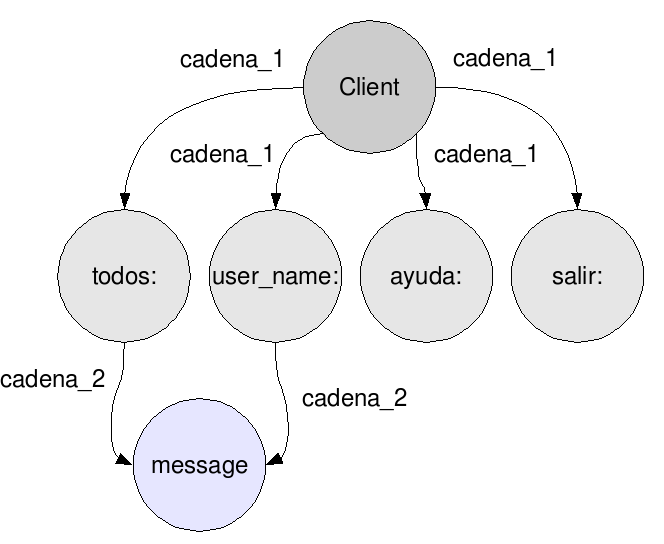
\includegraphics[scale=0.4]{user_actions.png}
				\caption{Comandes disponibles a executar per un client connectat a un servidor.}
				\label{user_actions}
				\end{center}
				\end{figure}

		\subsubsection{Protocol client-servidor}
		En la següent llista enumerada veurem els detalls del protocol que s'ha d'implementar entre un client i un servidor; aquest consta de les següents característiques:
			\begin{enumerate}
			\item El servidor espera connexions en el port \emph{TCP/8642}.
			\item El client passarà de forma iterativa per les següents etapes:
				\begin{enumerate}
				\item Estat de configuració (veure secció \ref{configuracio}).
				\item Estat de connexió; el client es connecta al servidor per el port \emph{TCP/8642} i el servidor espera el missatge d'identificació. Si es produeix algun error el client finalitza la sessió.
				\item Estat d'identificació; consta de:
					\begin{enumerate}
					\item El client envia un missatge d'identificació i espera el missatge \emph{OK} del servidor.
					\item El servidor envia el missatge \emph{OK} i entra en espera del missatge de registre.
					\end{enumerate}
				\item Estat de registre; consta de:
					\begin{enumerate}
					\item El client envia un missatge de registre.
					\item El servidor dóna d'alta a l'usuari , (desant l'identificador del mateix, l'adreça \emph{IP} des de la qual es connecta i el port \emph{UDP} d'on rebrà els missatges privats), envia un missatge \emph{OK} i entra en un bucle d'espera de peticions.
					\end{enumerate}
				Registrar-se amb un identificador d'usuari present actualment en el sistema, es considera un error. Quan s'acaba la connexió amb un client pel motiu que sigui, aquest es donarà de baixa en el registre.
				\item Estat de peticions al servidor; consta de:
					\begin{enumerate}
					\item Missatge pregunta, el client demana l'adreça \emph{IP} d'un usuari i el port \emph{UDP} pel qual es rebran els missatges provats. El servidor respon amb un missatge resposta. Si l'usuari no existeix el servidor enviarà com adreça \emph{IP} ``\emph{null}'' i el port \emph{UDP} 0.
					Nota: el client iniciarà pel seu compte una comunicació amb el client en el port \emph{UDP} i adreça \emph{IP} obtingudes.
					\item Missatge de difusió, es demana al servidor que envïi un missatge a tots els clients connectats actualment. El servidor envia a tots els usuaris connectats (excepte al de la font del missatge de difusió) i envia un missatge \emph{OK} a l'emisor un cop satisfeta la petició.
					\item Missatge de sortir, s'informa al servidor de l'eixida de la sessió.
					\end{enumerate}
				\end{enumerate}
			\end{enumerate}
		Observacions generals:
			\begin{enumerate}
 			\item Si no es cumpleix el protocol per part del client, ja sigui perque el missatge enviat és sintàcticament o semànticament incorrecte, el servidor envia un missatge \emph{ERROR} al client i finalitza la sessió amb el mateix.
 			\item Si no es cumpleix el protocol per part del servidor, ja sigui perque el missatge enviat és sintàcticament o semànticament incorrecte, el client envia un missatge \emph{SALIR} al servidor i el client finalitza la sessió.
 			\item La recepció d'un missatge \emph{ERROR} obliga al client a finalitzar la sessió.
 			\item L'enviament d'un missatge \emph{SALIR} per part del client obliga a aquest a finalitzar la sessió.
 			\item Si el client detecta que el servidor ha caigut, finalitza la sessió.
 			\item Si el servidor detecta que el client ha caigut o bé rep un missatge \emph{SALIR}, finalitza la sessió amb el client, això implica donar de baixa a l'usuari enregistrat.
 			\item Qualsevol altra situació no contemplada en aquest protocol tan en el servidor com en el client porta a finalitzar la sessió ja sigui en el servidor o en el client.
 			\item No hi ha \emph{timeouts}.
			\end{enumerate}

		\subsubsection{Protocol client-client}
		Un client pot enviar un missatge privat a un altre client (usuari) després que el primer hagi obtingut l'adreça \emph{IP} i el port \emph{UDP} del segon, a través del servidor. Un cop obtinguda l'adreça, s'envia un missatge privat. Així doncs, els clients poden rebre missatges tant per la connexió establerta amb el servidor com pel port \emph{UDP} que han indicat l'usuari.\\
		Tots aquests missatges es mostraran a l'usuari i s'especificarà la font.\\
		Observació: qualsevol recepció pel port \emph{UDP} que no correspongui a un missatge privat, serà descartat automàticament.

		\subsubsection{Missatges}
		La sintaxis dels missatges que estan permesos en aquest protocol, es poden veure en l'esquema de la figura \ref{missatges}.

		        \begin{figure}[h]
			\begin{center}
			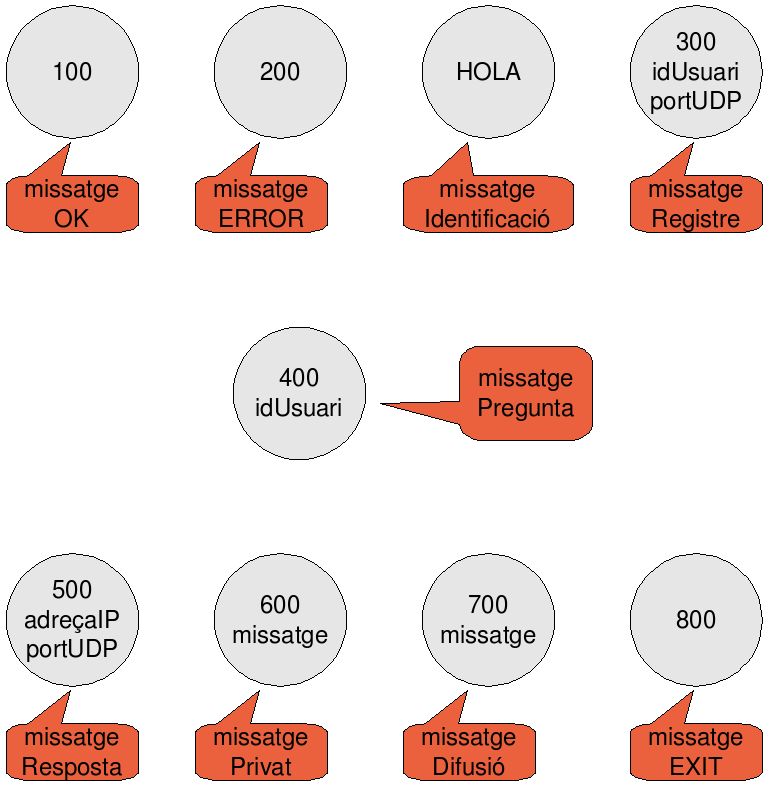
\includegraphics[scale=0.4]{messages.png}
			\caption{Missatges operatius en un client.}
			\label{missatges}
			\end{center}
			\end{figure}

	\subsection{Metodologia de treball}
	En aquest apartat es fa un breu resum de la metodologia de treball que s'ha adoptat per resoldre la pràctica, és a dir, llenguatge de programació i eines usades pel desenvolupament de la pràctica.

		\subsubsection{Per què \emph{python} i \emph{c++} ?}
		Tal i com podrà apreciar el nostre \emph{rewiever} la pràctica ha estat implementada usant dos llenguatges de programació: \emph{c++} i \emph{python}. Per què proposem dos dissenys? Doncs bé, lluny de la teoria que apunta que el fet de programar amb dos llenguatges diferents suposa incrementar exponencialment el volum de feina, nosaltres proposem una metodologia basada en la implementació en \emph{python} per la posterior ``traducció'' a \emph{c++} tal i com es mostra en l'esquema de la figura \emph{metod}.

			\begin{figure}[h]
			\begin{center}
			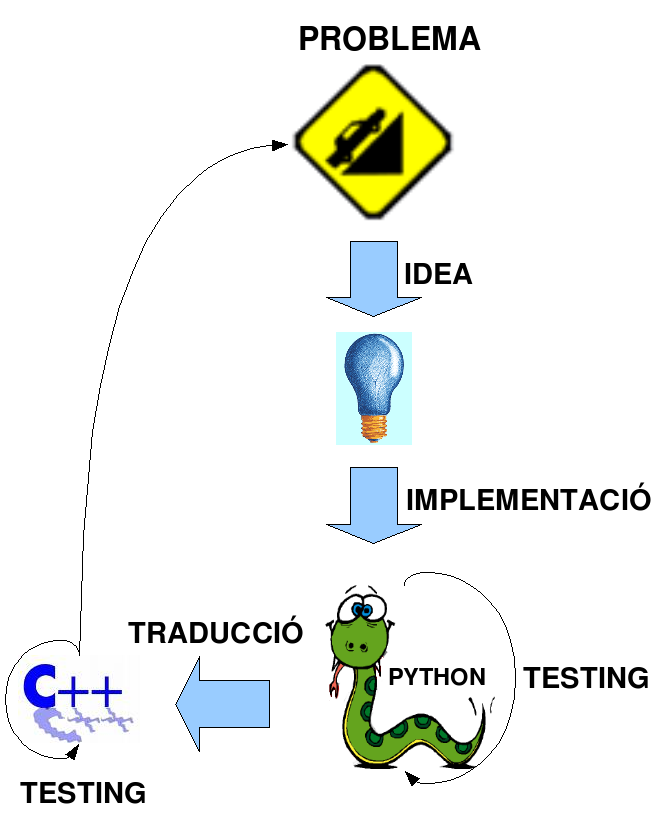
\includegraphics[scale=0.4]{metode.png}
			\caption{Mètode d'implementació.}
			\label{metod}
			\end{center}
			\end{figure}

		El pas de traducció no es gens complicat, ja que l'estructura d'ambdós llenguatges és força semblant; a més a més el fet d'usar un disseny modular basat en classes facilita molt l'addesió poc a poc de les capes que formaran tota la implementació de la pràctica (en \emph{python} i \emph{c++}).

		\subsubsection{Eines usades}
		Aquesta pràctica s'ha desenvolupat en un entorn format per tres desenvolupadors (els tres integrants del grup). La necessitat de coordinar la feina entre nosaltres suposava un repte important, ja que una bona organització de grup facilitaria molt les coses i evitaria la realització de feina inútil, replicada \ldots o d'altres malentesos entre nosaltres.

		Així doncs, per tal que tots nosaltres tinguéssim accés durant tot el dia al codi font (i d'altres arxius de la pràctica) hem creat un repositori \emph{Subversion} amb 3 usuaris per tal que sigui el gestor de versions el que s'encarregui de resoldre els conflictes existents entre les versions que s'han portat a terme.

		Pel que fa a l'eina de programació, cada integrant del grup ha usat el que li ha semblat més oportú, usant des de \emph{Kwrite} a \emph{Kate} o \emph{Vim}.

		La documentació del codi s'ha realitzat usant l'eina \emph{Doxygen}\footnote{\emph{Doxygen} és un generador de documentació per \emph{c++}, \emph{c}, \emph{java}, \emph{objective-C}, \emph{python} \ldots entre altres. Degut a la seva fàcil adaptació, funciona amb la majoria de sistemes \emph{Unix}, així com en \emph{Windows} i \emph{Mac Os X}. La major part del codi està desenvolupada per \emph{Dimitri van Heesch}.} mentre que aquest informe s'ha desenvolupat usant el llenguatge \LaTeX. Les imatges que s'han creat s'han dissenyat usant \emph{oodraw} i el sistema operatiu que s'ha usat en el desenvolupament de la pràctica han estat les distribucions \emph{Linux} \emph{Debian} i \emph{K-Ubuntu Edgy Eft}.

\section{Disseny de la pràctica}
En aquest apartat, és comentaran els trets principals de les classes que formen tota la implementació en \emph{python}. Un cop s'hagin repassat totes les classes d'aquesta implementació, es comentaran els trets diferenciadors entre ambdues versions.

	\subsection{Disseny de classes en \emph{python}}
	En aquesta subsecció farem un repàs dels punts més importants del disseny efectuat amb \emph{python}. L'ordre en que els diferents mòduls es van succeïnt en l'execució d'una connexió entre el servidor i un client ve esquematitzat en la figura \ref{piram_py}.
			\begin{figure}[h]
			\begin{center}
			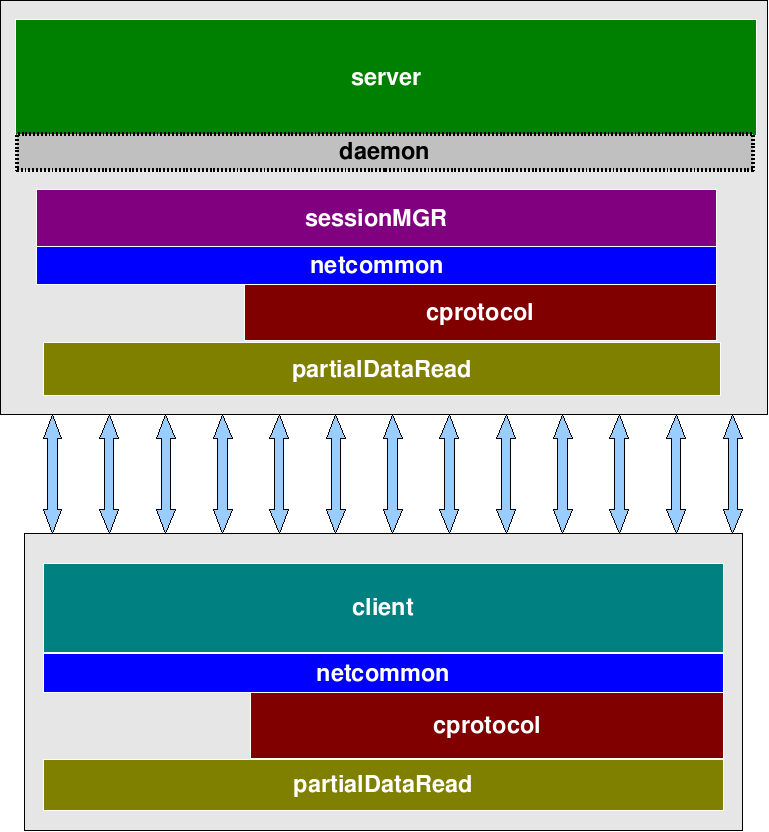
\includegraphics[scale=0.35]{piramide_py.png}
			\caption{Diagrama de seqüència de les classes implementades en \emph{python}.}
			\label{piram_py}
			\end{center}
			\end{figure}

 	Així doncs en aquesta figura es mostra que:
		\begin{enumerate}
		\item \textcolor{red}{[S]}: S'executa el mòdul \emph{server}.
		\item \textcolor{red}{[S]}: S'executa (o depèn de l'usuari) el mòdul \emph{daemon}.
		\item \textcolor{blue}{[C]}: S'executa un client.\\
		Associat a l'execució del client tindrem que un seguit de mòduls es posaran en funcionament en ambdós parts, és a dir, en la banda del servidor \emph{server} i del client \emph{client}.
		\item \textcolor{red}{[S]}: S'executa el mòdul \emph{sessionMGR}.
		\item \textcolor{red}{[S]}\&\textcolor{blue}{[C]}: S'executa el mòdul \emph{netcommon}.
		\item \textcolor{red}{[S]}\&\textcolor{blue}{[C]}: S'executa el mòdul \emph{cprotocol}.
		\item \textcolor{red}{[S]}\&\textcolor{blue}{[C]}: S'executa el mòdul \emph{partialDataRead}.
		\end{enumerate}
	On \textcolor{red}{[S]} significa que s'executa des del servidor, \textcolor{blue}{[C]} que s'executa des del client i \textcolor{red}{[S]}\&\textcolor{blue}{[C]} que s'executa des d'ambdós punts.

	Així doncs, entre l'esquema de la figura \ref{piram_py} i l'enumeració anterior, es pot arribar a entrendre que un disseny basat en la implementació de funcionalitats en classes, era la via òptima per afrontar de forma coherent i elegant la problemàtica de la pràctica, ja que l'ús d'un disseny modular ens permet que els diferents agregats o classes tinguin certa independència, la qual cosa ens habilita la reutilització de gran quantitat de codi i ens dóna com a resultat una aplicació molt robusta i coherent.

	Un cop comentem el per què de l'existència de classes, anem a veure de forma molt breu els mòduls existents i la seva funcionalitat. Així doncs tindrem:
		\begin{itemize}
		\item Mòdul \emph{server}: conté la classe \emph{server}, encarregada de la realització de tasques per tal de realitzar serveis en benefici dels clients que es connectin a ell.
		\item Mòdul \emph{daemon}: en aquest mòdul s'implementa la funció \emph{daemon()} de \emph{c++} que ens permet executar el servidor en mode \emph{background} (o \emph{dimoni}) en la nostra implementació en \emph{python}, ja que en aquest llenguatge no existeix aquest mètode.\\
		Aquest mòdul és tracta d'una nova funcionalitat que s'ha afegit a la implementació de la pràctica.
		\item Mòdul \emph{sessionMGR}: conté la classe \emph{sessionMGR} i \emph{clientSession} que són usades de forma exclusiva per el mòdul \emph{server} per tal de gestionar (creació i destrucció) de les sessions dels clients (\emph{clientSession}), és a dir, dels clients pròpiament dits i la informació associada: identificador, adreça \emph{IP} \ldots etc.
		\item Mòdul \emph{netcommon}: conté referències a la classe \emph{selectInterface}. Aquestes referències són usades pels mòduls arrel \emph{server} i \emph{client} que els utilitzen per treballar amb els descriptors de fitxer dels diferents clients.
		\item Mòdul \emph{cprotocol}: és el mòdul que conté la implementació de la gramàtica que han de seguir client i servidor. A més a més de definir els possibles estats d'un client, també és un mòdul que s'usa cada vegada que s'ha d'enviar i processar un missatge, és a dir, en les classes \emph{client}, \emph{server} i \emph{clientSession} (es troba dins de \emph{sessionMGR}).
		\item Mòdul \emph{partialDataRead}: és la classe usada pel client i el servidor quan aquests es troben en estat d'espera de dades, és a dir, és la classe que s'encarrega de les lectures parcials.
		\item Mòdul \emph{client}: conté la classe \emph{client}, encarregada de realitzar aquelles tasques que ens permetran accedir als serveis que ens ofereix el servidor i així comunicar-nos amb d'altres usuaris (o clients) del servei.
		\end{itemize}

	\subsection{Disseny de classes en \emph{c++}}
	Seguint la mateixa metodologia i basant-se en el següent diagrama de seqüència de les classes que formen la implementació en \emph{c++} (mostra't en la figura \ref{piram_c}), comentarem en aquest cas, però, les diferències més significatives que hi ha entre la versió \emph{python} i \emph{c++}, ja que com hem comentat anteriorment segueixen la mateixa estructura.

			\begin{figure}[h]
			\begin{center}
			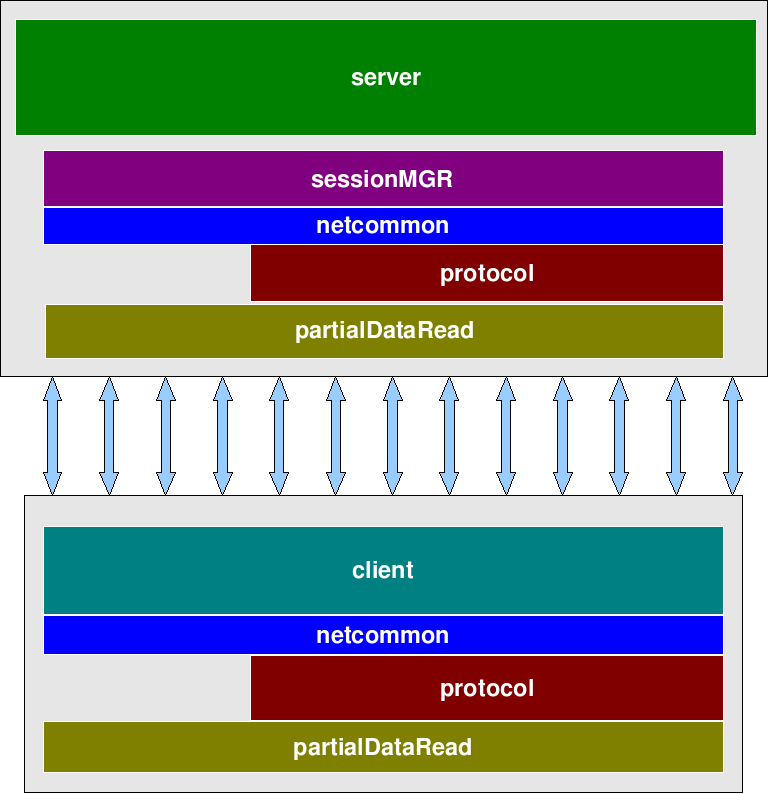
\includegraphics[scale=0.35]{piramide_c.png}
			\caption{Diagrama de seqüència de les classes implementades en \emph{c++}.}
			\label{piram_c}
			\end{center}
			\end{figure}

	La diferència fonamental que volem destacar entre el disseny \emph{python} i \emph{c++} és la manera en què s'usa l'operació \emph{select}.

	En ambdues versions tota la funcionalitat del \emph{select} es troba encapsulada dins de la classe \emph{selectInterface} (dins de \emph{netcommon}), que ens permet evitar errors ja que amb aquest encapsulament el programador no té la responsabilitat de comprovar si \emph{fdmax} conté un valor correcte, de calcular-lo \ldots etc; ja que és la classe \emph{selectInterface} la qui s'ocupa de fer-ho, reduïnt al màxim la possibilitat que aquest cometi un error. Dit en alt nivell, és una manera d'automatitzar el funcionament de \emph{select} treient feina al desenvolupador.

	Mentre en \emph{python} aquest encapsulament treballa amb objectes la qual cosa és més elegant i polimòrfic, en la versió de \emph{c++} es treballa directament amb els descriptors de fitxers la qual cosa resulta més farragós i menys abstracte.

	\subsection{Cas particular: lectures parcials}
	El punt que ens va comportar molts problemes, fou el referent a les lectures parcials, com podiem llegir dades incompletes i enviar-les i tenir en compte els separadors de línia.

	A continuació comentarem dos punts molt importants que ens han permés posar remei a aquests problemes.

		\subsubsection{partialDataReader}
		Aquest mòdul ens va permetre llegir dades que no eren completes, és a dir, que eren parcials, acumular-les en un registre per tal d'unir-les amb la resta de dades que manquen per tractar-les tan bon punt es rebia el separador de línia.

		\subsubsection{Separador de línia}
		La problemàtica dels caràcters separadors de línia i els protocols d'internet, és el fet que a part dels missatges, també s'envien peticions que són de caracter protocolari. Així doncs, s'havia de controlar com marcavem el final de cada línia.
		
		Usar el conegut ``\emph{$\setminus$n}'' del \emph{c++} era perillós en la implementació \emph{python}. Així doncs vam decidir-nos per usar com a separador els caràcters ``\emph{$\setminus$r$\setminus$n}'' ja que és la implementació usada de forma estàndard en tots els protocols on s'intercanvia text pla\footnote{Veure \url{http://www.rfc-editor.org/EOLstory.txt}.} (com en el nostre cas). Aquesta solució és més flexible del que sembla, ja que també es permet rebre dades amb separadors de tot tipus: ``\emph{$\setminus$n}'', ``\emph{$\setminus$r}'' i ``\emph{$\setminus$r$\setminus$n}'', per tal d'acceptar aquelles implementacions que segons el nostre punt de vista no són del tot correctes.


	\subsection{Màquina d'estat del client}
	En aquesta secció es mostra de forma esquemàtica una màquina d'estats (emulant les màquines d'autòmats) on es pot veure els diferents estats en què un client es pot trobar, i com depenent dels missatges aquest client es trobarà dins d'un estat o dins d'un altre.

		\begin{figure}[h]
		\begin{center}
		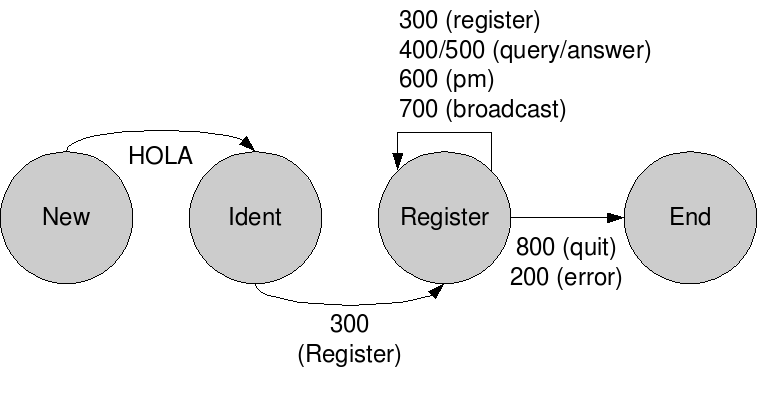
\includegraphics[scale=0.5]{automat.png}
		\caption{Màquina d'estats del client.}
		\label{estat}
		\end{center}
		\end{figure}

	\subsection{Manuals d'execució}
	En aquest apartat mostrarem com s'han d'executar ambdues versions de la pràctica, és a dir, les crides que s'han de portar a terme, els arguments (si en tenen) \ldots etc, per tal que la pràctica funcioni correctament.

		\subsubsection{Versió \emph{python}}
		Un cop estiguem ubicats dins de la carpeta del codi implementat en python \emph{/python}, haurem d'executar el servidor. Per fer-ho teclejarem:
			\begin{verbatim}
			./server.py 
			\end{verbatim}
		Aquesta seria una execució sense cap paràmetre, però el nostre servidor permet la parametrització de certs valors, que són:
			\begin{itemize}
			\item \emph{-p $<$port$>$}; per tal d'establir un port \emph{TCP} determinat (per defecte 8642).
			\item \emph{-b $<$backlog$>$}; per tal d'establir el nombre de connexions en cua en mode espera (per defecte 10).
			\item \emph{-D}; una nova funcionalitat que ens permet fer córrer el servidor en mode \emph{background} o dimoni (per defecte desactivat).
			\item \emph{-buf $<$size$>$}; per tal d'establir el tamany del buffer d'entrada (per defecte 4096).
			\item \emph{-nw}; per activar l'opció d'ignorar els espais en blanc en els noms d'usuari (per defecte activat)
			\item \emph{-bind $<$address$>$}; per tal d'establir adreces a connexió (per defecte s'accepten totes les adreces disponibles per totes les interfícies: ``0'').
			\item \emph{-ctt}; per tal de netejar els caràcters \emph{$<$IAC$>$}, \emph{$<$TOF$>$} i \emph{$<$OPT$>$} del protocol \emph{telnet} (per defecte desactivat).
			\item \emph{-e}; permet que hi hagi ``\emph{cmds}'' buits des del client (per defecte desactivat).
			\item \emph{--help}; per mostrar l'ajuda.
			\end{itemize}

		Un cop ja tenim el servidor en funcionament, és el moment d'executar un client, per fer-ho teclejarem dins de la metaixa carpeta \emph{/python} el següent:
			\begin{verbatim}
			./client.py 
			\end{verbatim}
		Aquesta seria una execució sense cap paràmetre, però els nostres clients permeten la parametrització de certs valors, que són:
			\begin{itemize}
			\item \emph{nick@server:port}; nom\_usuari@adreça\_\emph{IP}:port\_\emph{TCP}.
			\item \emph{-p $<$port$>$}; per tal d'establir un port \emph{UDP} determinat (per defecte assignat aleatòriament pel sistema operatiu).
			\item \emph{-buf $<$size$>$}; per tal d'establir el tamany del buffer d'entrada (per defecte 4096).
			\item \emph{-bind $<$address$>$}; per tal d'establir adreces a connexió (per defecte s'accepten totes les adreces disponibles per totes les interfícies: ``0'').
			\item \emph{--help}; per mostrar l'ajuda.
			\end{itemize}

		\subsubsection{Versió \emph{c++}}
		Un cop estiguem ubicats en el directori del codi implementat en \emph{c++}, caldrà compilar tots els fitxers, per fer-ho teclejarem:
			\begin{verbatim}
 			make
			\end{verbatim}
		Aquesta comanda cridarà al nostre \emph{Makefile} i ens generarà els executables del client i servidor. Per executar el nostre servidor implementat en \emph{c++} teclejarem:
			\begin{verbatim}
			./server
			\end{verbatim}
		Aquesta seria una execució sense cap paràmetre, però el nostre servidor permet la parametrització de certs valors, que són:
			\begin{itemize}
			\item \emph{-p $<$port$>$}; per tal d'establir un port \emph{TCP} determinat (per defecte 8642).
			\item \emph{-b $<$backlog$>$}; per tal d'establir el nombre de connexions en cua en mode espera (per defecte 10).
			\item \emph{-D}; ens permet fer córrer el servidor en mode \emph{background} o dimoni (per defecte desactivat).
			\item \emph{--help}; per mostrar l'ajuda.
			\end{itemize}
		Un cop ja tenim el servidor en funcionament, és el moment d'executar un client, per fer-ho teclejarem dins de la meteixa carpeta el següent:
			\begin{verbatim}
			./client 
			\end{verbatim}
		Aquesta seria una execució sense cap paràmetre, però els nostres clients permeten la parametrització de certs valors, que són:
			\begin{itemize}
			\item \emph{nick@server:port}; nom\_usuari@adreça\_\emph{IP}:port\_\emph{TCP}.
			\item \emph{-p $<$port$>$}; per tal d'establir un port \emph{UDP} determinat (per defecte 0).
			\item \emph{--help}; per mostrar l'ajuda.
			\end{itemize}

\pagebreak
\section{Eina de testing}
En aquesta secció explicarem com hem portat a terme les proves als nostres servidors.
	
	\subsection{testool.py}	
	El testing està basat en un script implementat en \emph{python} anomenat \emph{testool.py}. Aquest script s'ha d'executar un cop tenim el servidor corrent, també és recomanable que hi hagi un client en funcionament que haurem de crear nosaltres mateixos i establir-li un port \emph{UDP} inferior al 7000, per exemple el 6999.
	
	Aquest script es llança amb la comanda:
	\begin{verbatim}
	./testtool.py argument1 argument2 argument3 argument4
	\end{verbatim}
	On tenim que:
		\begin{itemize}
		\item El primer argument correspon al nom d'usuari que s'usarà per crear el client dins del test.
		\item El segon argument correspon a l'adreça \emph{IP} que volem usar en la connexió.
		\item El tercer argument és el port \emph{UDP} per el qual es volen rebre/enviar els missatge privats.
		\item El quart argument indica el nombre de missatges a enviar pel client.
		\end{itemize}
	Per tal d'entrendre millor els arguments anem a explicar que fa concretament aquest script:
	
	El script crea un client amb identificador \emph{argument1} que el que farà és enviar \emph{argument4}x2 (ja que envia la cadena \emph{``Eggs!!''} i la cadena \emph{``Spam!!''} per separat) missatges de broadcast (\emph{todos: missatge}) des de l'adreça \emph{IP} \emph{argument2} pel port \emph{UDP} \emph{argument3}. Un cop enviats tots els missatges, aquest client de testing enviarà el missatge \emph{SALIR} i es desconnectarà del servidor.

	\subsection{test.sh}
	Una altra eina de test més exhaustiva és la que s'ha implementat en el \emph{script} \emph{test.sh}. Aquest \emph{script} està basat amb l'anterior \emph{script} \emph{testool.py}.

	Aquesta eina de testeig \emph{test.sh} el que porta a terme és una crida mitjançant un bucle de 100 execucions de \emph{testool.py}. Però, com s'ha resolt la crida del script inicial amb paràmetres? Doncs bé, fem un cop d'ull al codi:
	\begin{verbatim}
	#!/bin/bash
	for i in `seq 1 100`; do
	    let port=7000+i
	    python testtool.py bep$i localhost $port 10 &
	done
	\end{verbatim}
	Tal i com es pot veure és porta a terme un bucle de 100 iteracions on es crida a \emph{testool.py} amb els arguments:
		\begin{itemize}
		\item Usuari \emph{bep\$i}; això significa que a cada volta de bucle, es crida a l'usuari \emph{bep1}, \emph{bep2}, \emph{bep3} \ldots i així fins \emph{bep100}.
		\item Adreça \emph{IP}  \emph{localhost} en totes les iteracions.
		\item Port \emph{UDP} \emph{\$port}, de la mateixa forma que en el cas dels usuaris, el port s'incrementa en una unitat per cada volta de bucle per tal d'evitar que la informació sigui molt caòtica a la resta de clients que ja formen part del xat. Es comença pel port 7000 i s'acabarà pel 7100.
		\item El nombre de missatges a enviar és 10, la qual cosa cada client enviarà 10 cops \emph{Eggs!!} i 10 cops \emph{Spam!!}.
		\end{itemize}

\pagebreak
\section{Conclusions}
En aquesta pràctica hem après diferents coses que han aportat molt a la nostra formació en aquesta assignatura, però també en tots els àmbits. 

Hem après a treballar amb equip i a utilitzar aquelles eines que ens permeten fer-ho. Hem ampliat els nostres coneixements en la temàtica de la pràctica, és a dir, amb la utilització de \emph{sockets}. També a criticar el treball fet mitjançant els tests que s'han creat per veure les possibilitats, capacitat i robustesa del nostre disseny. També s'ha realitzat un treball força interessant i molt sovint inexistent ens molts projectes de software com és la realització de documentació del mateix, en aquest cas en dos àmbits: codi font a mesura que aquest s'implementava i també de la documentació recopilatòria final (aquest informe) per tal d'expressar els trets generals de tot el que ha envoltat el desenvolupament d'aquesta pràctica.

Esperem també, més endavant, aprendre a realitzar avaluacions objectives de les propostes d'altri quan portem a terme el \emph{peer review} i a comparar ambdós dissenys per tal de veure les mancances o avantatges tan del nostre disseny com el de l'altre grup.

En definitiva un conjunt d'aprenentatges que pensem que són molt interessants, ja que engloben totes les etapes que un bon desenvolupament de software ha de tenir, en el nostre cas, de software lliure.

\pagebreak
\section{Llicència del document}
Obra subjecte a una llicència de Reconeixement-Compartir amb la mateixa llicència 2.5 Espanya Creative Commons. Per veure'n una còpia visiteu: \url{http://creativecommons.org/licenses/by-sa/2.5/es/} o bé envieu una carta a:\\
        \begin{center}
        Creative Commons\\
        559 Nathan Abbott Wayy\\
        Stanford\\
        California 94305\\
        USA
        \end{center}

\end{document}